\documentclass{standalone}
\usepackage{tikz}
\usetikzlibrary{shapes.geometric,patterns.meta}

\begin{document}
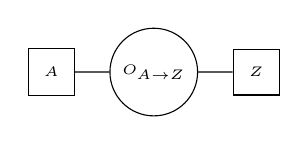
\begin{tikzpicture}[square/.style={regular polygon,regular polygon sides=4}]
    \node at (0, 0) [circle, minimum size=0.8cm, draw] (cir) {\tiny $O_{A \rightarrow Z}$};
    \node at (-1.3, 0) [square, draw] (s) {\tiny $A$};
    \node at (1.3, 0) [square, draw] (e) {\tiny $Z$};

    \draw (s.east) -- (cir.west); 
    \draw (cir.east) -- (e.west); 
\end{tikzpicture}
\end{document}
